\beginsong{Der Pfahl}[
    wuw={Lluís Llach}, 
    jahr={1968},
    txt={Oss Kröher (Übersetzung)},
    pfiii={56}, 
    gruen={24}, 
    siru={218}, 
    tonspur={476}, 
    buedel={278},
    index={Sonnig begann es zu tagen},
]

\beginverse
\endverse
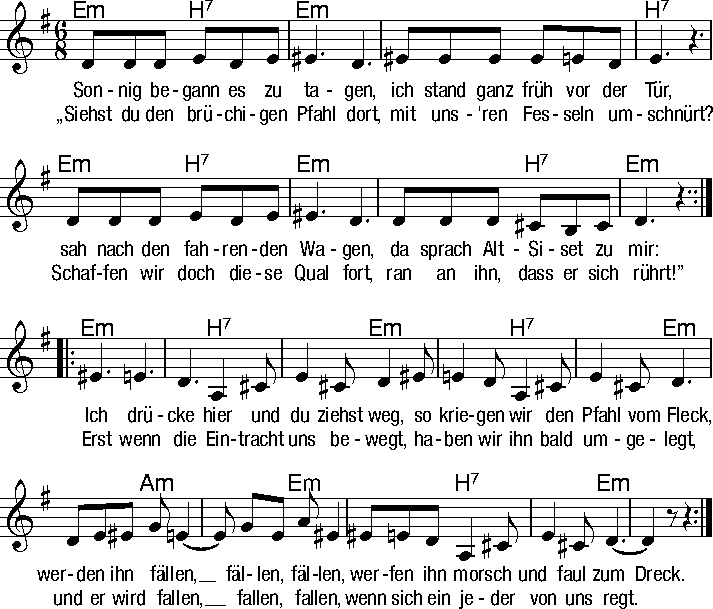
\includegraphics[draft=false, width=1\textwidth]{Noten/Lied018.pdf}	

\beginverse
\[Em]'Ach Siset, \[H7]noch ist es \[Em]nicht geschafft, an meiner Hand platzt die \[H7]Haut.
\[Em]Langsam auch \[H7]schwindet schon \[Em]meine Kraft, er ist zu \[H7]mächtig ge\[Em]baut.
Wird es uns \[H7]jemals ge\[Em]lingen? Siset, es fällt mir so \[H7]schwer!'
\[Em]'Wenn wir das \[H7]Lied nochmal \[Em]singen, geht es viel \[H7]besser. Komm \[Em]her!'
\endverse

\beginchorus 
\[Em]Ich drücke \[H7]hier und du ziehst \[Em]weg, so kriegen \[H7]wir den Pfahl vom \[Em]Fleck,
werden ihn \[Am]fällen, fällen, \[Em]fällen, werfen ihn \[H7]morsch und faul zum \[Em]Dreck.
Erst wenn die \[H7]Eintracht uns be\[Em]wegt, haben wir \[H7]ihn bald umge\[Em]legt
und er wird \[Am]fallen, fallen, \[Em]fallen, wenn sich ein \[H7]jeder von uns \[Em]regt!
\endchorus

\beginverse
^Der alte ^Siset sagt ^nichts mehr, böser Wind hat ihn ver^weht.
^Keiner weiß ^von seiner ^Heimkehr, keiner weiß, ^wie es ihm ^geht.
Alt-Siset ^sagte uns ^allen, hör es auch du, krieg es ^mit:
^Der morsche ^Pfahl wird schon ^fallen, wie es ge^schieht in dem ^Lied.
\endverse

\beginchorus
\[Em]Ich drücke \[H7]hier und du ziehst \[Em]weg, so kriegen \[H7]wir den Pfahl vom \[Em]Fleck,
werden ihn \[Am]fällen, fällen, \[Em]fällen, werfen ihn \[H7]morsch und faul zum \[Em]Dreck.
Erst wenn die \[H7]Eintracht uns be\[Em]wegt, haben wir \[H7]ihn bald umge\[Em]legt
und er wird \[Am]fallen, fallen, \[Em]fallen, wenn sich ein \[H7]jeder von uns \[Em]regt!
Und er wird \[Am]fallen, fallen, \[Em]fallen, wenn sich ein \[H7]jeder von uns \[Em]regt!
\endchorus

\endsong

\beginscripture{}
Das Lied ist die Übersetzung von L'estaca von Luis Lach. Der Pfahl ist hier Sinnbild für den Staat. Das Lied ist zur Zeit der Diktatur in Katalonien bekannt geworden.
\endscripture
